\documentclass[11pt,a4paper]{article}
\usepackage[utf8]{inputenc}
\usepackage{hyperref}
\usepackage{minted}
\usepackage{tikz}

\usepackage{todonotes}

\title{Introducing Bluetooth Low Energy}
\author{Kolbjørn Austreng}
\date{}

\begin{document}
\maketitle

\renewcommand{\thesection}{\roman{section}}
\renewcommand{\thesubsection}{\roman{section}.\alph{subsection}}

\section{Introduction}
Wired protocols are all well and nice - and although CAN is a relatively old protocol now partly superseded by CAN-FD (ISO 11898); it is still widely used today. Nevertheless, wireless protocols are becoming increasingly popular wherever they can be used, due to their low cost, and ease of use.\\
\\
One such protocol - Bluetooth Low Energy, or Bluetooth 4.2 (BLE for short) - is almost certainly supported by your smart phone; as well as a plethora of different devices, prevalent in our daily life. This makes it an ideal candidate for introducing wireless connectivity to your project - provided you can live with the interference present in the ISM band.\\
\\
Many of the students taking this course will previously have had the course "Embedded Systems" (TTK4235), in which the "BBC micro:bit" development board was used during the labs. This is an excellent platform for introducing the Bluetooth Low Energy stack, and we will be using the micro:bit platform in this course as well. TTK4235 is no prerequisite, and it should be straight forward to follow this lab assignment without having gone through that course.\\
\\
If no one on your group has a micro:bit, you may talk to one of the student assistants. It is also possible to use other hardware, such as an nRF52 development kit if you happen to have one, but bear in mind that other hardware platforms support different Application Programming Interfaces (APIs) for the Bluetooth stack.\\
\\
Beware: This lab assignment has been written for- and tested on Linux. Since Mac is Unix based, you should be able to follow relatively painlessly if you happen to be an Apple Sheeple. It is probably possible to do this using Windows as well, if you identify as a masochist - but no guarantees ;)

\newpage
\noindent
\section{Initial Setup of Hardward and Toolchain}
The following hardware configuration is only necessary for those of you who have not already done so through TTK4235. However, it might still be necessary to set up the toolchain, as nothing is certain when it comes to the computers at the real time lab.

\subsection{Hardware Configuration}
By default, the micro:bit comes preloaded with a custom Device Abstraction Layer (DAL) that allows programming the device through Scratch, Micropython, or JavaScript. This is well for simple demonstrations, but yields no control of the low level hardware. To get around this limitation, we will upgrade the flasher circuit to use the BBC micro:bit J-Link OB Firmware.

\begin{enumerate}
\item Download the \href{https://www.segger.com/downloads/jlink#BBC\_microbit}{J-Link OB Firmware from Segger.com}\footnote{https://www.segger.com/downloads/jlink\#BBC\_microbit}.
\item Start with the micro:bit unplugged. While holding down the Reset button (next to the USB connector), connect it to the computer.
\item The micro:bit should now have mounted itself as "MAINTENANCE" on the file system. You can now let go of the Reset button.
\item Move the .hex-file that you downloaded into "MAINTENANCE".
\item The micro:bit should now automatically remount after a few seconds; this time as "MICROBIT".
\end{enumerate}

\subsection{Toolchain Configuration}
\label{sec::toolchain_config}
To compile and flash code for the micro:bit, we need to install a toolchain. For compilation, GCC is a natural choice. Since the heart of the micro:bit is an nRF51822, we will be using J-Link and nrfjprog to flash the board.

\begin{enumerate}
\item Call \mintinline{text}{nrfjprog --version} to see if the toolchain is already set up on the computer. If it is, you may skip the remaining steps.
\item Call \mintinline{text}{sudo apt install gcc-arm-none-eabi} to install the GCC ARM compiler.
\item Go to \href{https://www.nordicsemi.com/eng/nordic/Products/nRF51822/nRF5x-Command-Line-Tools-Linux64/51386}{nordicsemi.com}\footnote{https://www.nordicsemi.com/eng/nordic/Products/nRF51822/nRF5x-Command-Line-Tools-Linux64/51386} and download the newest version of the nRF command line tools.
\item The download contains the programs \mintinline{text}{nrfjprog} and \mintinline{text}{mergehex}, both must be available in the Linux \mintinline{text}{PATH} variable. This can be done in many ways, here is one:
\begin{enumerate}
\item Extract the \mintinline{text}{nrfjprog}- and \mintinline{text}{mergehex} folders to the home folder.
\item Add the following string at the bottom of the \mintinline{text}{~/.bashrc} file: \mintinline{bash}{"export PATH=$HOME/nrfjprog:$HOME/mergehex:$PATH"} (do not include the quotation marks)%$
\item Finally, since \mintinline{text}{~/.bashrc} is read once when a terminal opens, you need to close and reopen all terminal windows that you might have active.
\end{enumerate}
\item Go to \href{https://www.segger.com/downloads/jlink/\#J-LinkSoftwareAndDocumentationPack}{segger.com}\footnote{https://www.segger.com/downloads/jlink/\#J-LinkSoftwareAndDocumentationPack} and download the J-Link Software and Documentation pack. You should choose the Linux 64 bit version, DEB installer.
\item Once you have downloaded the DEB package, navigate to the download location with a terminal, and call the following command to install the package: \mintinline{text}{sudo dpkg -i JLink_Linux[...]x86_64.deb}
\end{enumerate}

\subsection{Hardware and Toolchain Verification}
First off, you should call \mintinline{text}{nrfjprog --version} to see if the toolchain is set up. If this command complains, you will need to repeat section \ref{sec::toolchain_config}.\\
\\
On Blackboard, you can find an example .hex-file that you can flash to the micro:bit to test that it works correctly. To use it, navigate to the directory where you have the hex, and call \mintinline{text}{nrfjprog -f nrf51 ...} \todo{Add example project}

\section{Use your phone for testing}
You are free to use whatever to check your Bluetooth connection, but an easy choice is to download the "nRF Connect" app for your smart phone. This lab assignment will use that app.\todo{Add app screenshots}

\newpage
\noindent
\setcounter{section}{0}
\renewcommand{\thesection}{\arabic{section}}
\renewcommand{\thesubsection}{\arabic{section}.\arabic{subsection}}

\section{Heads up}
Bluetooth Low Energy (BLE) is a messy beast to tackle, so it might be smart to skim appendix \ref{app::intro_ble} as you go through this lab assignment. Don't fret if you do not get all the details however - some things are better understood when coded, rather than when read.\\
\\
Finally, an honest word from the author of this assignment: Sometimes, the Nordic Semi documentation can be a little "Meh". Feeling like there should be a more elegant way to do Bluetooth Low Energy is completely normal - and you are advised to simply bite the pillow when the going gets rough.\\
\\
Do enjoy :)

\section{First steps - GAP}
The 

\newpage
\noindent
\appendix
\section{Introduction to BLE}
\label{app::intro_ble}
\begin{figure}
\centering
\resizebox{\linewidth}{!}{
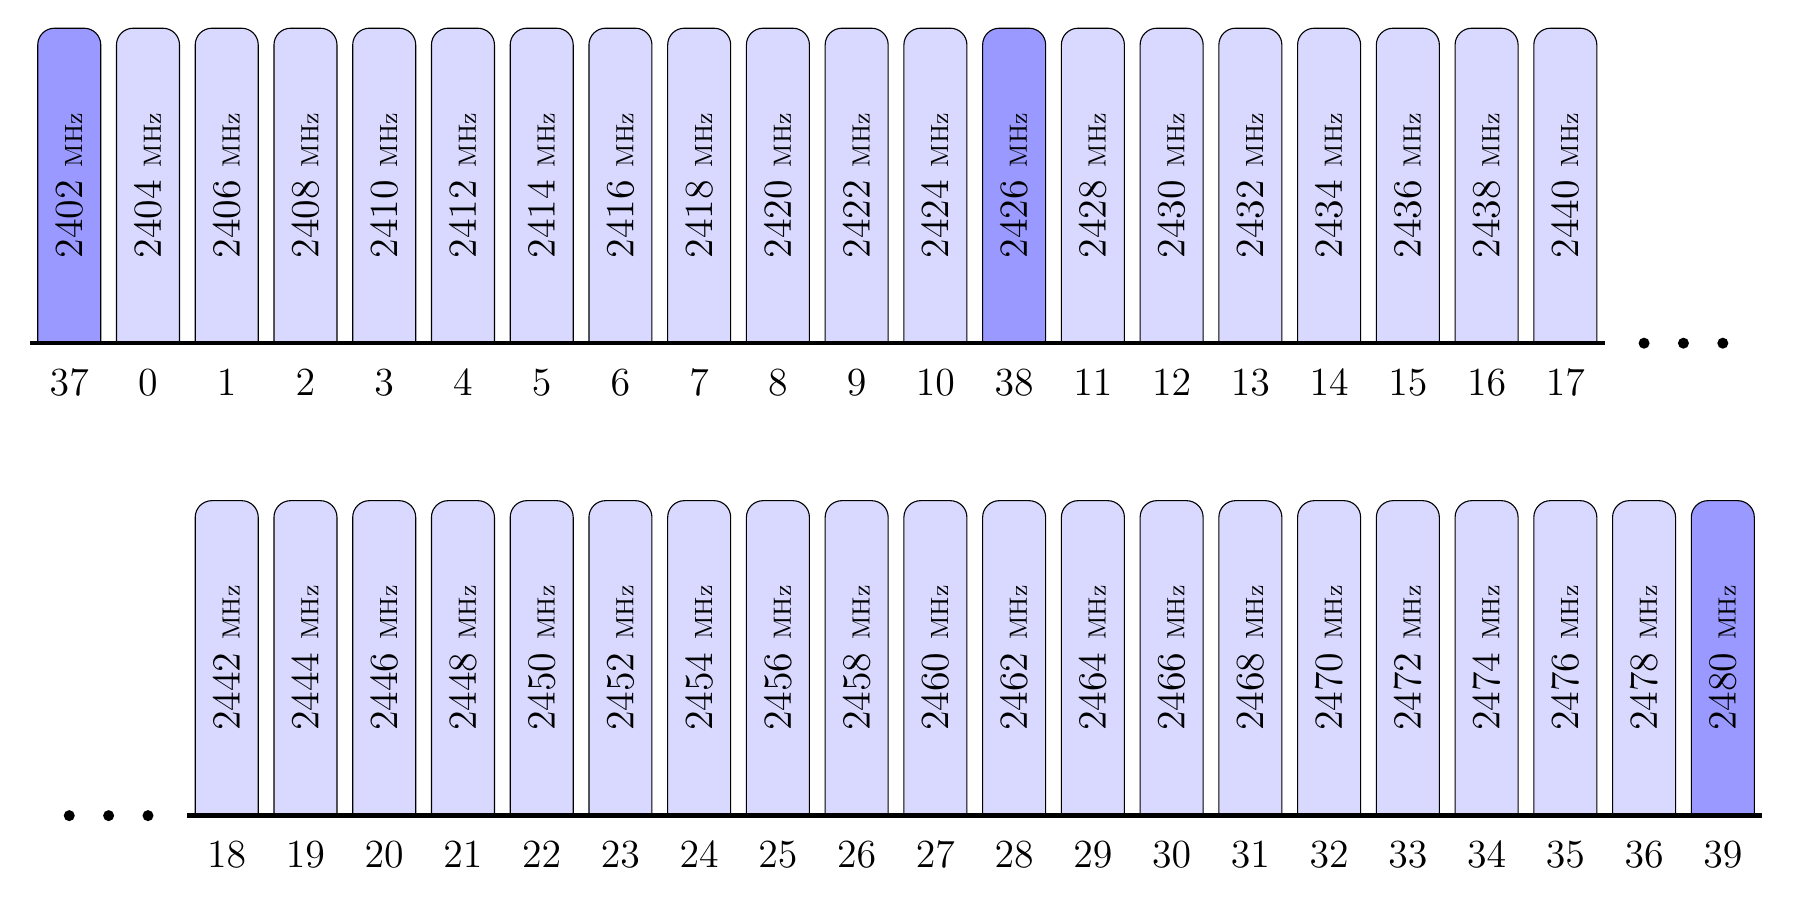
\begin{tikzpicture}
\colorlet{regular_channel_fill}{blue!15}
\colorlet{advertise_channel_fill}{blue!40}

\foreach \x in {0,1,...,19}{
\fill[regular_channel_fill,rounded corners=0.6em](\x + 0.1, 0) -- ++(0,4) -- ++(0.8,0) -- ++(0,-4);
}
\foreach \x in {0,12}{
\fill[advertise_channel_fill,rounded corners=0.6em](\x + 0.1, 0) -- ++(0,4) -- ++(0.8,0) -- ++(0,-4);
}
\foreach \x in {0,1,...,19}{
\pgfmathsetmacro{\f}{int(2402 + 2 * \x)}
\draw[rounded corners=0.6em] (\x + 0.1,0) -- ++(0,4) -- ++(0.8,0) -- ++(0,-4);
\path (\x,0) rectangle ++(1,4) node[midway,rotate=90] {\Large$\f$ \small MHz};
}
\foreach \x/\ch in {0/37,1/0,2/1,3/2,4/3,5/4,6/5,7/6,8/7,9/8,10/9,11/10,12/38,13/11,14/12,15/13,16/14,17/15,18/16,19/17}{
\path (\x,-1) rectangle ++(1,1) node[midway] {\Large\ch};
}
\draw[ultra thick] (0,0) -- ++(20,0);
\foreach \x in {1,1.5,2}{
\fill (19.5 + \x, 0) circle [radius=0.07];
}

% Line two
\begin{scope}[xshift=-18cm, yshift=-6cm]
\foreach \x in {20,21,...,39}{
\fill[regular_channel_fill,rounded corners=0.6em](\x + 0.1, 0) -- ++(0,4) -- ++(0.8,0) -- ++(0,-4);
}
\fill[advertise_channel_fill,rounded corners=0.6em](39 + 0.1,0) -- ++(0,4) -- ++(0.8,0) -- ++(0,-4);
\foreach \x in {20,21,...,39}{
\pgfmathsetmacro{\f}{int(2402 + 2 * \x)}
\draw[rounded corners=0.6em] (\x + 0.1,0) -- ++(0,4) -- ++(0.8,0) -- ++(0,-4);
\path (\x,0) rectangle ++(1,4) node[midway,rotate=90] {\Large$\f$ \small MHz};
}
\foreach \x/\ch in {20/18,21/19,22/20,23/21,24/22,25/23,26/24,27/25,28/26,29/27,30/28,31/29,32/30,33/31,34/32,35/33,36/34,37/35,38/36,39/39}{
\path (\x,-1) rectangle ++(1,1) node[midway] {\Large\ch};
}
\draw[ultra thick] (20,0) -- ++(20,0);
\foreach \x in {1,1.5,2}{
\fill (17.5 + \x, 0) circle [radius=0.07];
}
\end{scope}
\end{tikzpicture}
}
\end{figure}
Blah blah


\end{document}